% Copied from:
% http://mirror.its.dal.ca/ctan/macros/latex/contrib/IEEEtran/bare_conf.tex
\documentclass[conference]{IEEEtran}
% Some Computer Society conferences also require the compsoc mode option,
% but others use the standard conference format.
%
% If IEEEtran.cls has not been installed into the LaTeX system files,
% manually specify the path to it like:
% \documentclass[conference]{../sty/IEEEtran}

\usepackage{changepage}





% Some very useful LaTeX packages include:
% (uncomment the ones you want to load)


% *** MISC UTILITY PACKAGES ***
%
%\usepackage{ifpdf}
% Heiko Oberdiek's ifpdf.sty is very useful if you need conditional
% compilation based on whether the output is pdf or dvi.
% usage:
% \ifpdf
%   % pdf code
% \else
%   % dvi code
% \fi
% The latest version of ifpdf.sty can be obtained from:
% http://www.ctan.org/pkg/ifpdf
% Also, note that IEEEtran.cls V1.7 and later provides a builtin
% \ifCLASSINFOpdf conditional that works the same way.
% When switching from latex to pdflatex and vice-versa, the compiler may
% have to be run twice to clear warning/error messages.






% *** CITATION PACKAGES ***
%
%\usepackage{cite}
% cite.sty was written by Donald Arseneau
% V1.6 and later of IEEEtran pre-defines the format of the cite.sty package
% \cite{} output to follow that of the IEEE. Loading the cite package will
% result in citation numbers being automatically sorted and properly
% "compressed/ranged". e.g., [1], [9], [2], [7], [5], [6] without using
% cite.sty will become [1], [2], [5]--[7], [9] using cite.sty. cite.sty's
% \cite will automatically add leading space, if needed. Use cite.sty's
% noadjust option (cite.sty V3.8 and later) if you want to turn this off
% such as if a citation ever needs to be enclosed in parenthesis.
% cite.sty is already installed on most LaTeX systems. Be sure and use
% version 5.0 (2009-03-20) and later if using hyperref.sty.
% The latest version can be obtained at:
% http://www.ctan.org/pkg/cite
% The documentation is contained in the cite.sty file itself.






% *** GRAPHICS RELATED PACKAGES ***
%
\ifCLASSINFOpdf
  \usepackage[pdftex]{graphicx}
  \usepackage{epstopdf}
  % declare the path(s) where your graphic files are
 \graphicspath{{diagrams/}}
  % and their extensions so you won't have to specify these with
  % every instance of \includegraphics
  \DeclareGraphicsExtensions{.pdf,.jpeg,.png,.eps}
\else
  % or other class option (dvipsone, dvipdf, if not using dvips). graphicx
  % will default to the driver specified in the system graphics.cfg if no
  % driver is specified.
  \usepackage[dvips]{graphicx}
  % declare the path(s) where your graphic files are
  \graphicspath{{diagrams/}}
  % and their extensions so you won't have to specify these with
  % every instance of \includegraphics
  \DeclareGraphicsExtensions{.eps}
\fi
% graphicx was written by David Carlisle and Sebastian Rahtz. It is
% required if you want graphics, photos, etc. graphicx.sty is already
% installed on most LaTeX systems. The latest version and documentation
% can be obtained at:
% http://www.ctan.org/pkg/graphicx
% Another good source of documentation is "Using Imported Graphics in
% LaTeX2e" by Keith Reckdahl which can be found at:
% http://www.ctan.org/pkg/epslatex
%
% latex, and pdflatex in dvi mode, support graphics in encapsulated
% postscript (.eps) format. pdflatex in pdf mode supports graphics
% in .pdf, .jpeg, .png and .mps (metapost) formats. Users should ensure
% that all non-photo figures use a vector format (.eps, .pdf, .mps) and
% not a bitmapped formats (.jpeg, .png). The IEEE frowns on bitmapped formats
% which can result in "jaggedy"/blurry rendering of lines and letters as
% well as large increases in file sizes.
%
% You can find documentation about the pdfTeX application at:
% http://www.tug.org/applications/pdftex





% *** MATH PACKAGES ***
%
%\usepackage{amsmath}
% A popular package from the American Mathematical Society that provides
% many useful and powerful commands for dealing with mathematics.
%
% Note that the amsmath package sets \interdisplaylinepenalty to 10000
% thus preventing page breaks from occurring within multiline equations. Use:
%\interdisplaylinepenalty=2500
% after loading amsmath to restore such page breaks as IEEEtran.cls normally
% does. amsmath.sty is already installed on most LaTeX systems. The latest
% version and documentation can be obtained at:
% http://www.ctan.org/pkg/amsmath





% *** SPECIALIZED LIST PACKAGES ***
%
%\usepackage{algorithmic}
% algorithmic.sty was written by Peter Williams and Rogerio Brito.
% This package provides an algorithmic environment fo describing algorithms.
% You can use the algorithmic environment in-text or within a figure
% environment to provide for a floating algorithm. Do NOT use the algorithm
% floating environment provided by algorithm.sty (by the same authors) or
% algorithm2e.sty (by Christophe Fiorio) as the IEEE does not use dedicated
% algorithm float types and packages that provide these will not provide
% correct IEEE style captions. The latest version and documentation of
% algorithmic.sty can be obtained at:
% http://www.ctan.org/pkg/algorithms
% Also of interest may be the (relatively newer and more customizable)
% algorithmicx.sty package by Szasz Janos:
% http://www.ctan.org/pkg/algorithmicx




% *** ALIGNMENT PACKAGES ***
%
%\usepackage{array}
% Frank Mittelbach's and David Carlisle's array.sty patches and improves
% the standard LaTeX2e array and tabular environments to provide better
% appearance and additional user controls. As the default LaTeX2e table
% generation code is lacking to the point of almost being broken with
% respect to the quality of the end results, all users are strongly
% advised to use an enhanced (at the very least that provided by array.sty)
% set of table tools. array.sty is already installed on most systems. The
% latest version and documentation can be obtained at:
% http://www.ctan.org/pkg/array


% IEEEtran contains the IEEEeqnarray family of commands that can be used to
% generate multiline equations as well as matrices, tables, etc., of high
% quality.




% *** SUBFIGURE PACKAGES ***
%\ifCLASSOPTIONcompsoc
%  \usepackage[caption=false,font=normalsize,labelfont=sf,textfont=sf]{subfig}
%\else
%  \usepackage[caption=false,font=footnotesize]{subfig}
%\fi
% subfig.sty, written by Steven Douglas Cochran, is the modern replacement
% for subfigure.sty, the latter of which is no longer maintained and is
% incompatible with some LaTeX packages including fixltx2e. However,
% subfig.sty requires and automatically loads Axel Sommerfeldt's caption.sty
% which will override IEEEtran.cls' handling of captions and this will result
% in non-IEEE style figure/table captions. To prevent this problem, be sure
% and invoke subfig.sty's "caption=false" package option (available since
% subfig.sty version 1.3, 2005/06/28) as this is will preserve IEEEtran.cls
% handling of captions.
% Note that the Computer Society format requires a larger sans serif font
% than the serif footnote size font used in traditional IEEE formatting
% and thus the need to invoke different subfig.sty package options depending
% on whether compsoc mode has been enabled.
%
% The latest version and documentation of subfig.sty can be obtained at:
% http://www.ctan.org/pkg/subfig




% *** FLOAT PACKAGES ***
%
%\usepackage{fixltx2e}
% fixltx2e, the successor to the earlier fix2col.sty, was written by
% Frank Mittelbach and David Carlisle. This package corrects a few problems
% in the LaTeX2e kernel, the most notable of which is that in current
% LaTeX2e releases, the ordering of single and double column floats is not
% guaranteed to be preserved. Thus, an unpatched LaTeX2e can allow a
% single column figure to be placed prior to an earlier double column
% figure.
% Be aware that LaTeX2e kernels dated 2015 and later have fixltx2e.sty's
% corrections already built into the system in which case a warning will
% be issued if an attempt is made to load fixltx2e.sty as it is no longer
% needed.
% The latest version and documentation can be found at:
% http://www.ctan.org/pkg/fixltx2e


%\usepackage{stfloats}
% stfloats.sty was written by Sigitas Tolusis. This package gives LaTeX2e
% the ability to do double column floats at the bottom of the page as well
% as the top. (e.g., "\begin{figure*}[!b]" is not normally possible in
% LaTeX2e). It also provides a command:
%\fnbelowfloat
% to enable the placement of footnotes below bottom floats (the standard
% LaTeX2e kernel puts them above bottom floats). This is an invasive package
% which rewrites many portions of the LaTeX2e float routines. It may not work
% with other packages that modify the LaTeX2e float routines. The latest
% version and documentation can be obtained at:
% http://www.ctan.org/pkg/stfloats
% Do not use the stfloats baselinefloat ability as the IEEE does not allow
% \baselineskip to stretch. Authors submitting work to the IEEE should note
% that the IEEE rarely uses double column equations and that authors should try
% to avoid such use. Do not be tempted to use the cuted.sty or midfloat.sty
% packages (also by Sigitas Tolusis) as the IEEE does not format its papers in
% such ways.
% Do not attempt to use stfloats with fixltx2e as they are incompatible.
% Instead, use Morten Hogholm'a dblfloatfix which combines the features
% of both fixltx2e and stfloats:
%
% \usepackage{dblfloatfix}
% The latest version can be found at:
% http://www.ctan.org/pkg/dblfloatfix




% *** PDF, URL AND HYPERLINK PACKAGES ***

\usepackage{url}
% url.sty was written by Donald Arseneau. It provides better support for
% handling and breaking URLs. url.sty is already installed on most LaTeX
% systems. The latest version and documentation can be obtained at:
% http://www.ctan.org/pkg/url
% Basically, \url{my_url_here}.




% *** Do not adjust lengths that control margins, column widths, etc. ***
% *** Do not use packages that alter fonts (such as pslatex).         ***
% There should be no need to do such things with IEEEtran.cls V1.6 and later.
% (Unless specifically asked to do so by the journal or conference you plan
% to submit to, of course. )


% correct bad hyphenation here
\hyphenation{op-tical net-works semi-conduc-tor}


\begin{document}
%
% paper title
% Titles are generally capitalized except for words such as a, an, and, as,
% at, but, by, for, in, nor, of, on, or, the, to and up, which are usually
% not capitalized unless they are the first or last word of the title.
% Linebreaks \\ can be used within to get better formatting as desired.
% Do not put math or special symbols in the title.
\title{Visualizing Project Evolution Through Abstract Syntax Tree Analysis}


% author names and affiliations
% use a multiple column layout for up to three different
% affiliations
%\author{\IEEEauthorblockN{Michael D. Feist \and Eddie Antonio Santos \and
%  Ian Watts \and Abram Hindle}
%\IEEEauthorblockA{Department of Computing Science\\
%University of Alberta\\
%Edmonton, Canada\\
%\{mdfeist,easantos,watts1,hindle1\}@ualberta.ca}}

% conference papers do not typically use \thanks and this command
% is locked out in conference mode. If really needed, such as for
% the acknowledgment of grants, issue a \IEEEoverridecommandlockouts
% after \documentclass

% for over three affiliations, or if they all won't fit within the width
% of the page, use this alternative format:
%
\author{\IEEEauthorblockN{Michael D. Feist,
Eddie Antonio Santos,
Ian Watts,
Abram Hindle}
\IEEEauthorblockA{Department of Computing Science\\
University of Alberta\\
Edmonton, Canada\\
\{mdfeist,easantos,watts1,hindle1\}@ualberta.ca}}



% use for special paper notices
%\IEEEspecialpapernotice{(Invited Paper)}




% make the title area
\maketitle

% As a general rule, do not put math, special symbols or citations
% in the abstract
\begin{abstract}
Analysing the changes in software repositories over time is difficult since changes come from different developers and affect different parts of a repository.
Individual commits provide the changed files, code diffs and a message.
However, when many commits are viewed as a group, the details are lost.
Currently there is a lack of tools for tracking the changes in a repository beyond simply looking at the number of commits of lines changed.
The commit information can be misleading since lines of code gives no indication of what was actually being worked on without careful examination of the changed code.
Providing a more comprehensive view of this information could provide deeper insights into how software projects evolve since changes to design and features are not clearly visible.

We present a novel tool for visualizing Java projects.
It provides more detailed information regarding all of the changes along the master branch of a project.
It visualizes changes in type usage over time for projects and developers and derives detailed statistics using the differences between Abstract Syntax Trees (ASTs).
We are tracking additions and deletions of declarations and invocations for each type.
The AST diff between commits is a reentrant algorithm that can be incrementally calculated as new commits are made.

Using this tool we show the changes in type coverage and other usage statistics over time in several popular repositories.
Type coverage information from the AST is compared to file coverage to check for correlation or if there is unique information provided by type information.
Potential uses for such a tool for managers and developers is discussed.
\end{abstract}

% no keywords




% For peer review papers, you can put extra information on the cover
% page as needed:
% \ifCLASSOPTIONpeerreview
% \begin{center} \bfseries EDICS Category: 3-BBND \end{center}
% \fi
%
% For peerreview papers, this IEEEtran command inserts a page break and
% creates the second title. It will be ignored for other modes.
\IEEEpeerreviewmaketitle



\section{Introduction}

The history and evolution of software repositories are often tracked by version control systems. The information is generally kept in the form of commits, which show the differences between each subsequent version of the software.  These services become vital for large projects since individual changes would be impossible to track manually. Large projects have thousands of individual changes made by many different developers. With more changes to look through, it becomes more difficult to see how a project is evolving over time since there is so much information to look through. Most hosting services for git repositories provide some basic tools for analysing projects over time, but too much information is lost due to the lack of fine grained details. The information regarding contributions from developers are also misleading since the number of commits and lines of code do not necessarily reflect meaningful changes to a repository.

In Java, a type can be a primitive type or an object reference. Primitive types are those that are built into the language such as an int or char. Object references point to instances of classes in memory which are defined in the project or through an included library. The types in a project represent the functionality available for a developer to work with. A large or complex project may have many different types, whereas a small project might only use a few. Different parts of a program are going to use different types and libraries. When writing or contributing to a project, the author’s choice of which part of the program to edit will in turn affect what types they end up working with.

Having advanced tools for analysing repositories would benefit many different parts of the software development process. Software management requires a high level understanding of the state of a repository and the changes being made which affect the functionality of the software. Tracking developer contributions in a less misleading way is also important for management since important contributions may be small and focused. Line difference only provide meaningful info when they are analysed by someone with familiarity with the source code being changed. Providing tools which bring more meaning to line differences would allow people less familiar with the code to understand changes being made. When large changes are made that cover many lines of code, it would also be useful to see how the change affects the software rather than a several thousand line diff.  Seeing how a project has changed over time is also vital for management since evaluating the state of completion of software can be very difficult.

Type information is useful for seeing what libraries and functions are being used.  When a part of code becomes deprecated, continuing to use it may lead to design or  security flaws. Viewing the type information of a change can show when deprecated classes are added or removed from a project as well as how many remain. 

\section{Related Work}

Robert Dyer \textit{et al.} \cite{Dyer:2014:MBA:2568225.2568295} mined AST nodes to study the use of new Java language features over time. (More in challenge paper)

Grechanik \textit{et al.} \cite{Grechanik:2010:EIL:1852786.1852801} examined the structure of Java programs mined from 2080 programs. This paper examined the breakdown of syntactic structures in open source repositories, however it does not consider per author statistics. 

Meyerovich and Rabkin \cite{Meyerovich:2013:EAP:2509136.2509515} surveyed developers and examined repositories to learn about language adoption and usage. Developers feel that certain language features are more important than others.

Parnin \textit{et al.} \cite{Parnin:2011:JGA:1985441.1985446} mined repositories to see how Java generics have been used in open source projects and found that generic usages were often introduced by a single developer in a project. Generics usage was also fairly narrow, with the primary use being collecting and traversing lists of objects.

Patrick Wagstrom \textit{et al.} \cite{Patrick:Wagstrom:2012} explored the roles that developers take in a networked, social development environments like GitHub. These role were defined as their level of contribution as well as the types of issues they dealt with. Developers will take on multiple roles in a project and will sometimes fulfill the same role across different projects

L\"{a}mmel \textit{et al.} \cite{Lammel:2011:LAA:1982185.1982471} used ASTs to examine the usage of APIs in Java projects. They find what APIs are popular as well as if they are used in a framework like manner.

\section{Methodology}

An Abstract Syntax Tree (AST) is a tree structure which represents a piece of code by breaking its syntactic constructs into a tree structure. Each node in the tree represents a syntactically valid chunk of code which can be contained in a parent node or broken up into child nodes. This captures the structure of the code in an abstract manner. When a change is made to a file, the difference will also appear in the AST. This means that the AST of revisions in code repositories can be compared to see what structures a developer is touching. 

The ASTs were generated using Spoon \cite{pawlak:hal-01169705}. Spoon is a tool for transforming and analysing Java source code. It breaks code up into a meta-model including AST. The model consists of three parts: structural elements, code elements and references to program elements. The Spoon model is convenient because it provides the structure for performing an AST diff while retaining the code elements for analysis afterwards. Spoon also preserves all type and library information, which is what we were interested in.

GumTree \cite{falleri:hal-01054552} is an algorithm which is used to compute the difference between two ASTs generated by Spoon. For new files and deleted files we did not use GumTree; we simply ran Spoon on the files and treated everything as an addition or deletion respectively.

Once we have the generated ASTs we were able to run through the trees and count the declarations and invocations for a given type. For invocations we also recorded the method call. These stats were then marked as additions or deletions. 
\\
\begin{adjustwidth}{2.5em}{0pt}
\#DECLARE $\vert$ INSERT $\vert$ java.net.URI $\vert$ 2 \\
\#DECLARE $\vert$ DELETE $\vert$ java.lang.String $\vert$ 2 \\
\end{adjustwidth}

\begin{figure}[!h]
\centering
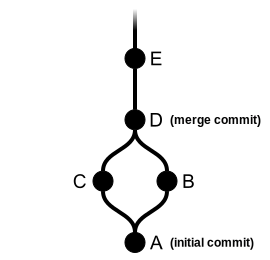
\includegraphics[height=2.5in]{commits_view}
\caption{The commits increase in time from bottom up. Therefore, B and C are compared against A and E is compared with D. Since D is a merge commit it is ignored as its changes are recorded in C and B.}
\end{figure}

In order to gather all the changes for a given repository over time we generated AST for each commit and compared the difference. We did this by running ‘git log’ over the git repository and listing all the commit ids in increasing time. Each commit and its parent were then compared. If the commit had no parent then every file in the commit was treated as an addition. Since we compared each commit to its parent we were able to account for branching that happened in the master branch of the repository. Also we ignored commits that were merges as all changes in the merge should already be accounted for in previous commits.

\begin{figure}[!h]
\centering
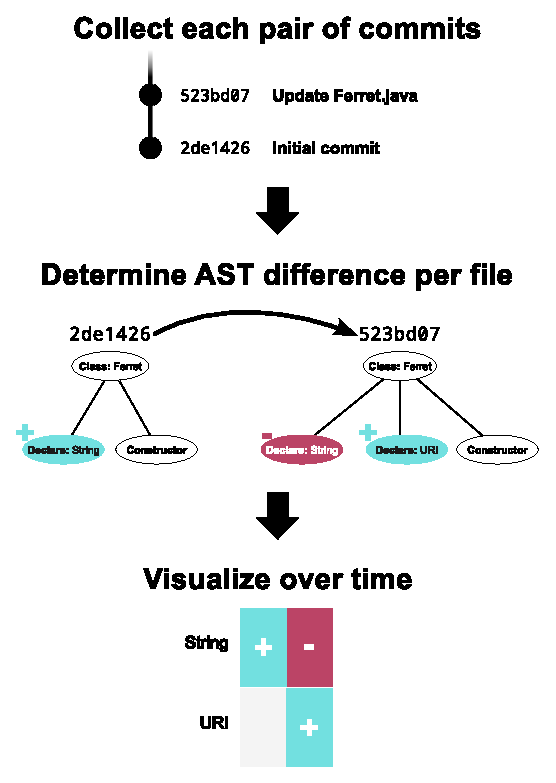
\includegraphics[width=\columnwidth]{context}
\caption{}
\end{figure}

\section{Case Study}

In the following sections, we present {N} case studies demonstrating the extra insight that TypeV makes available. 

\subsection{antlr4}

We chose Antlr4 as it is a substantial Java project, with a commit history spanning several years. We can also see distinct changes throughout its history.

For example, in December of 2011 we can see that ParserATNSimulator has a large amount of additions and deletions in roughly equal proportion (Figure~\ref{fig:parser1}. This suggests that ParserATNSimulator is not being removed from the project but instead there is some refactoring being done. If we take a closer look at the commit messages we can see that they mention refactoring and reorganization of code (Figure~\ref{fig:parser2}). Zooming in on that date,  shows that during that month they were finishing work on a new version of ParserATNSimulator. 

If we tried to do the same analyses with the GitHub tools it would be significantly more difficult to achieve the same conclusion. First if we only look at line changes this change to ParserATNSimulator is overwhelmed by other changes and hardly shows up on the GitHub tools. Then if we did notice an increase in activity we would not know what types were being worked on. Finally we could not quickly look at the commit messages for that specific time and type.

At certain times we can can see major increases across all types. This shows us when major changes to the code were being done versus code maintenance. Usually this happens when a large amount of code is being pulled in from another location.

\subsection{Apache Bookkeeper}

For deprecation analysis, we chose Apache Bookkeeper. As an Apache Foundation project it is a well-curated example of an open source software project. It also demonstrates an instance of deprecated methods. 

Apache Bookkeeper deprecated the method AbstractConfiguration.getLedgerManagerType() in release 4.2.0~\footnote{\url{https://bookkeeper.apache.org/docs/r4.2.0/apidocs/deprecated-list.html}} and replaced it with AbstractConfiguration.getLedgerManagerFactoryClass(). If we look at getLedgerManagerType() we can see at the time of the start of the deprecation all instances were removed and getLedgerManagerFactoryClass() was added. After the deprecation, we see no more changes to getLedgerManagerType() and only some additions of getLedgerManagerFactoryClass().

\section{Evaluation}

\section{Discussion}

\section{Conclusion}
The conclusion goes here.




% conference papers do not normally have an appendix


% use section* for acknowledgment
\section*{Acknowledgment}


The authors would like to thank...





% trigger a \newpage just before the given reference
% number - used to balance the columns on the last page
% adjust value as needed - may need to be readjusted if
% the document is modified later
%\IEEEtriggeratref{8}
% The "triggered" command can be changed if desired:
%\IEEEtriggercmd{\enlargethispage{-5in}}

% references section

% can use a bibliography generated by BibTeX as a .bbl file
% BibTeX documentation can be easily obtained at:
% http://mirror.ctan.org/biblio/bibtex/contrib/doc/
% The IEEEtran BibTeX style support page is at:
% http://www.michaelshell.org/tex/ieeetran/bibtex/
\nocite{*}
\bibliographystyle{IEEEtran}
% argument is your BibTeX string definitions and bibliography database(s)
\bibliography{bibliography,autogen}



% that's all folks
\end{document}
